%\documentclass[a4paper]{article}
%\usepackage[ampersand]{easylist}
%\usepackage{parskip}
%\usepackage{graphicx}
%\begin{document}

\part{Présentation de la société EdgeMind}
\chapter{L'entreprise}

\section{Présentation}
EdgeMind a été créée le 13 janvier 2014 par Roland Donat et Thomas  Friedlhuber sous la forme d’une SAS. Le 1er septembre 2016, ils sont rejoints par Vincent Leblond. Ces trois personnes constituent à la fois l’équipe dirigeante de la société et les experts techniques.

\begin{easylist}
\ListProperties(Hide=100, Hang=true, Progressive=3ex, Style*=--)
& ~Roland Donat : Président ;
& ~Thomas Friedlhuber : Directeur Général ;
& ~Vincent Leblond : Directeur commercial et projets.
\end{easylist}

L’actionnariat est détenu à 100\% par ces trois personnes physiques, salariées de la société et dont l’activité professionnelle est entièrement consacrée au développement de EdgeMind.

\section{Ressources humaines}

\begin{minipage}{0.7\textwidth}

À ce jour, EdgeMind se compose de 10 personnes localisées à Vannes, Nantes et Paris :
\begin{easylist}
\ListProperties(Hide=100, Hang=true, Progressive=3ex, Style*=--)
& ~7 salariés en CDI (dont l’équipe dirigeante) ;
& ~1 salariés en contrat d’apprentissage ;
& ~2 stagiaires de fin d’études niveau BAC+5.
\end{easylist}

\end{minipage}%
%
\begin{minipage}{0.4\textwidth}
\begin{center}
	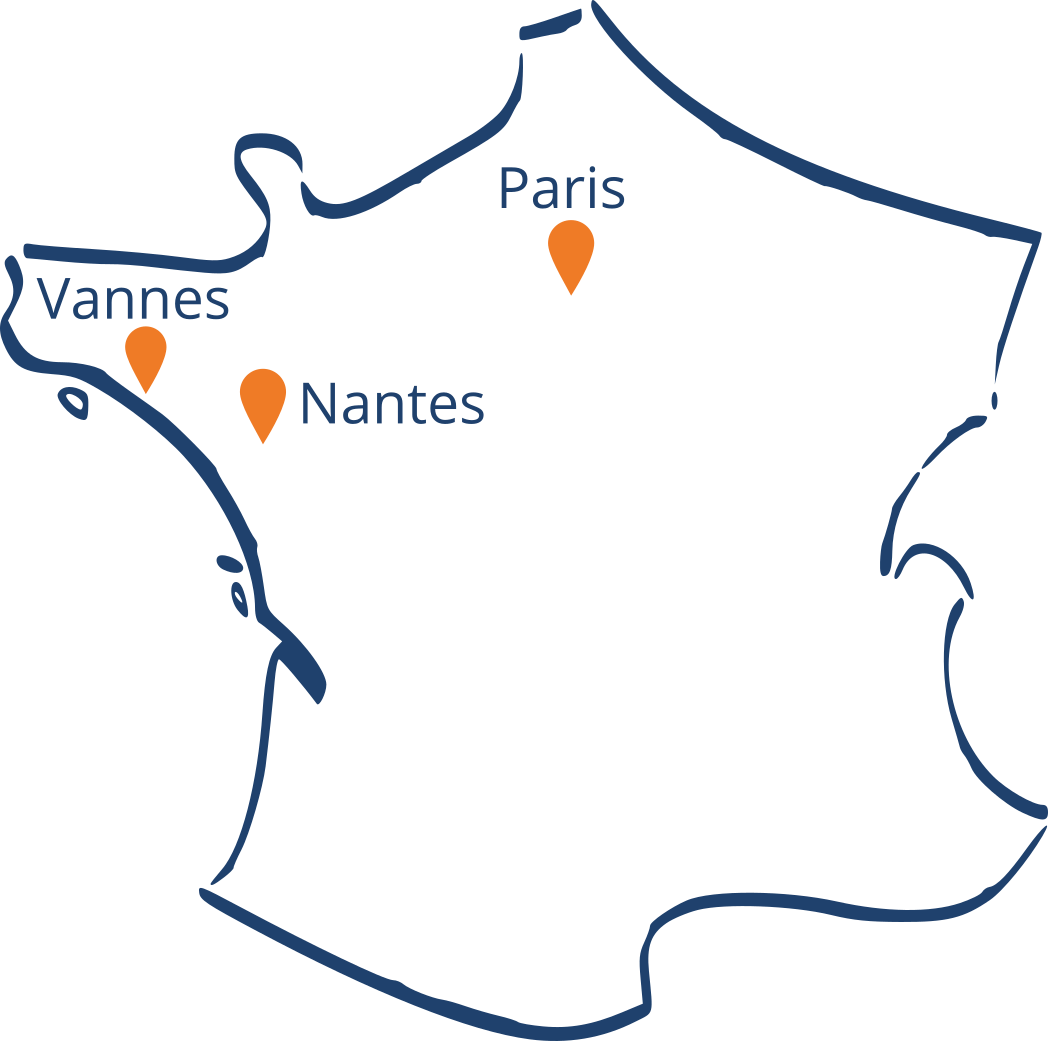
\includegraphics[scale=0.1]{figures/mini_france.png}
    \label{img:g}
\end{center}
\end{minipage}

Les compétences techniques du personnel couvrent :
\begin{easylist}
\ListProperties(Hide=100, Hang=true, Progressive=3ex, Style*=--)
& ~l’informatique scientifique ;
& ~la data science, machine learning et data visualisation ;
& ~la simulation multi-agent et la simulation de systèmes complexes ;
& ~l’analyse et la maîtrise des risques industriels ;
& ~la conception et la planification de systèmes de transport ;
& ~la recherche opérationnelle et l’optimisation ;
& ~le développement informatique desktop ;
& ~le développement informatique web ;
& ~la réalisation d’études et de prestations de conseil.
\end{easylist}

\section{Valeurs}

EdgeMind promeut et défend plusieurs valeurs dans ses relations commerciales et partenariales :
\begin{easylist}
\ListProperties(Hide=100, Hang=true, Progressive=3ex, Style*=--)
& ~Transparence ;
& ~Innovation et recherche scientifique ;
& ~Écoute des besoins métiers ;
& ~Relation de confiance ;
& ~Indépendance de ses activités.
\end{easylist}

\chapter{Activité}
\clearpage
\section{Activités, partenaires R\&D et clients}

EdgeMind est une société indépendante spécialisée dans l’innovation scientifique. Son activité repose sur la commercialisation de prestations et d’outils informatiques pour l’aide à la décision et l’optimisation de la performance opérationnelle. Ses secteurs d’activités privilégiés sont les transports, l’énergie et les territoires.

Les activités de EdgeMind couvrent les domaines de la maintenance prédictive, la maîtrise des risques industriels, la simulation des systèmes de transports et la valorisation des données métiers.

Les partenaires R\&D et les clients sont listés ci-dessous :

\begin{center}

\includegraphics[width=1\textwidth]{figures/clients_logo.png}
\end{center}

\section{Activités de recherche et innovation}

EdgeMind consacre plus de 50\% de son activité à la Recherche et Développement afin de constamment faire évoluer ses solutions et répondre aux besoins de ses clients. Nous cherchons également à débloquer les verrous scientifiques rencontrés lors de nos projets en nous appuyant sur nos liens avec des chercheurs issus d’instituts de recherche académique ou de l’industrie. Il est à noter que la société EdgeMind bénéficie du statut de Jeune Entreprise Innovante.

En 2018, EdgeMind a décidé d’investir avec ses fonds propres à hauteur de 160 K€ dans un projet de recherche partenarial au sein de l’Institut de Recherche Technologique System X. Ce projet sera réalisé sur une durée de 4 ans. Les grands objectifs de ce projet sont les suivants :
\begin{easylist}
\ListProperties(Hide=100, Hang=true, Progressive=3ex, Style*=--)
& ~spécifier et structurer les données opérationnelles afin d’identifier et formaliser les sources de données nécessaires à l’analyse des stratégies de maintenance ;
& ~améliorer le diagnostic des défaillances à partir de données complexes et hétérogènes ;
& ~modéliser les processus de maintenance prévisionnelle et déployer la chaîne d’outils associés sur des cas tests industriels ;
& ~élaborer une méthodologie générale pour la simulation et l’évaluation technico-économique des politiques de maintenance;
& ~développer des algorithmes d’optimisation globale des stratégies de maintenance en incluant les processus de soutien logistique associés.
\end{easylist}

Les partenaires du projet sont des industriels du secteur de l’énergie, de l’aéronautique et du transport.

\begin{center}

\includegraphics[width=1\textwidth]{figures/clients_logo2.png}
\end{center}

\begin{center}

\includegraphics[width=1\textwidth]{figures/clients_logo2bis.png}
\end{center}

%\end{document}